\documentclass[12pt,a4paper]{article}

% ─── Page Layout ───────────────────────────────────────────────────────────────
\usepackage[a4paper, margin=0.8in, headheight=14pt]{geometry}

% ─── Fonts (XeLaTeX) ───────────────────────────────────────────────────────────
\usepackage{fontspec}
\usepackage{unicode-math}
\setmainfont{TeX Gyre Pagella}
\setmonofont[Scale=0.88]{TeX Gyre Cursor}
\setmathfont{Latin Modern Math}

% ─── Packages ──────────────────────────────────────────────────────────────────
\usepackage{xcolor}
\usepackage{colortbl}
\usepackage{titlesec}
\usepackage{enumitem}
\usepackage{tabularx}
\usepackage{booktabs}
\usepackage{array}
\usepackage{amsmath}
\usepackage{tikz}
\usetikzlibrary{shapes.geometric, arrows.meta, positioning, calc, fit, decorations.pathreplacing}
\usepackage{tcolorbox}
\tcbuselibrary{skins, breakable}
\usepackage{hyperref}
\usepackage{fancyhdr}
\usepackage{graphicx}
\usepackage{microtype}
\hyphenpenalty=10000
\exhyphenpenalty=10000
\sloppy
\usepackage{caption}
\usepackage{setspace}
\usepackage{multirow}
\usepackage{tocloft}

% ─── Q&A helper ────────────────────────────────────────────────────────────────
\newcommand{\Q}[1]{\textbf{#1}\par\noindent\ignorespaces}

% ─── Colour Palette ────────────────────────────────────────────────────────────
\definecolor{myred}{RGB}{196,30,58}
\definecolor{mydark}{RGB}{30,30,50}
\definecolor{mygreen}{RGB}{14,120,80}
\definecolor{myteal}{RGB}{0,130,140}
\definecolor{myamber}{RGB}{180,100,0}
\definecolor{mypurple}{RGB}{100,30,160}
\definecolor{mygray}{RGB}{246,247,249}
\definecolor{mgframe}{RGB}{180,185,200}
\definecolor{watermark}{RGB}{145,150,170}
\definecolor{hdrred}{RGB}{250,232,235}
\definecolor{hdrgreen}{RGB}{220,244,233}
\definecolor{hdrteal}{RGB}{220,242,244}
\definecolor{hdramber}{RGB}{253,242,215}
\definecolor{hdrpurple}{RGB}{238,228,255}
\definecolor{hdrgray}{RGB}{238,240,245}
\definecolor{rowalt}{RGB}{250,251,253}

% ─── Section Formatting ────────────────────────────────────────────────────────
\titleformat{\section}
  {\large\bfseries\color{myred}}{\thesection.}{0.5em}{}
  [\vspace{1pt}{\color{myred}\rule{\linewidth}{0.8pt}}]
\titleformat{\subsection}
  {\normalsize\bfseries\color{myteal}}{\thesubsection}{0.5em}{}
\titlespacing*{\section}{0pt}{18pt}{7pt}
\titlespacing*{\subsection}{0pt}{11pt}{4pt}

% ─── Paragraph ─────────────────────────────────────────────────────────────────
\setlength{\parindent}{0pt}
\setlength{\parskip}{4pt}

% ─── TOC Styling ───────────────────────────────────────────────────────────────
\renewcommand{\cfttoctitlefont}{\large\bfseries\color{myred}}
\renewcommand{\cftaftertoctitle}{\par\noindent{\color{myred}\rule{\linewidth}{0.8pt}}}
\setlength{\cftbeforetoctitleskip}{0pt}
\setlength{\cftaftertoctitleskip}{6pt}
\renewcommand{\cftsecfont}{\normalsize\bfseries\color{mydark}}
\renewcommand{\cftsecpagefont}{\normalsize\bfseries\color{mydark}}
\renewcommand{\cftsecleader}{\cftdotfill{\cftdotsep}}
\setlength{\cftbeforesecskip}{7pt}
\renewcommand{\cftsubsecfont}{\small\color{mydark}}
\renewcommand{\cftsubsecpagefont}{\small\color{mydark}}
\setlength{\cftbeforesubsecskip}{3pt}
\setlength{\cftsubsecindent}{1.4em}

% ─── Table helpers ─────────────────────────────────────────────────────────────
\renewcommand{\arraystretch}{1.45}
\setlength{\tabcolsep}{6pt}
\arrayrulecolor{mydark}
\newcolumntype{B}[1]{>{\small\bfseries\raggedright\arraybackslash}m{#1}}
\newcolumntype{Y}{>{\small\raggedright\arraybackslash}X}
\renewcommand{\tabularxcolumn}[1]{m{#1}}

% ─── Header / Footer ───────────────────────────────────────────────────────────
\pagestyle{fancy}
\fancyhf{}
\fancyhead[L]{\small\color{myred}\textbf{PE-EC702B}\;\color{mydark}--- Digital Image and Video Processing}
\fancyhead[R]{\small\color{myteal}\textbf{Module 7 Notes}}
\fancyfoot[C]{\small\color{mydark}\thepage}
\fancyfoot[R]{\small\color{watermark}\textit{\copyright\ Biraj}}
\renewcommand{\headrulewidth}{0.5pt}
\renewcommand{\footrulewidth}{0.3pt}

% ─── Hyperref ──────────────────────────────────────────────────────────────────
\hypersetup{
  colorlinks=true, linkcolor=myteal, urlcolor=myteal,
  pdfauthor={Biraj Sarkar},
  pdftitle={PE-EC702B --- Module 7 Notes}
}

% ─── tcolorbox styles ──────────────────────────────────────────────────────────
\tcbset{
  tikzbox/.style={
    colback=mygray, colframe=mgframe, boxrule=0.6pt, arc=4pt,
    left=8pt, right=8pt, top=6pt, bottom=6pt,
    colbacktitle=mgframe, coltitle=mydark,
    fonttitle=\small\bfseries
  },
  defbox/.style={
    colback=hdrgreen, colframe=mygreen, boxrule=0.8pt, arc=4pt,
    left=9pt, right=9pt, top=6pt, bottom=6pt,
    colbacktitle=mygreen, coltitle=white,
    fonttitle=\small\bfseries
  },
  formulabox/.style={
    colback=hdrteal, colframe=myteal, boxrule=0.8pt, arc=4pt,
    left=9pt, right=9pt, top=7pt, bottom=7pt,
    colbacktitle=myteal, coltitle=white,
    fonttitle=\small\bfseries
  },
  examplebox/.style={
    colback=hdramber, colframe=myamber, boxrule=0.8pt, arc=4pt,
    left=9pt, right=9pt, top=6pt, bottom=6pt,
    colbacktitle=myamber, coltitle=white,
    fonttitle=\small\bfseries,
    breakable
  },
  masonbox/.style={
    colback=hdrpurple, colframe=mypurple, boxrule=0.8pt, arc=4pt,
    left=9pt, right=9pt, top=6pt, bottom=6pt,
    colbacktitle=mypurple, coltitle=white,
    fonttitle=\small\bfseries
  },
  exambox/.style={
    colback=hdrpurple, colframe=mypurple, boxrule=1pt, arc=5pt,
    left=10pt, right=10pt, top=8pt, bottom=8pt,
    colbacktitle=mypurple, coltitle=white,
    fonttitle=\bfseries,
    breakable, title after break={\textbf{Frequently Asked / Viva Questions (contd.)}}}
}
\tcbset{breakable}

% ─── TikZ styles ───────────────────────────────────────────────────────────────
\tikzset{
  block/.style={rectangle, draw=myteal, fill=hdrteal,
    text width=2.1cm, align=center, minimum height=0.85cm,
    font=\small, rounded corners=3pt, line width=0.7pt},
  arrow/.style={-Stealth, thick, color=mydark},
  line/.style={thick, color=mydark}
}

% ═══════════════════════════════════════════════════════════════════════════════
\begin{document}
% ═══════════════════════════════════════════════════════════════════════════════

\begin{center}
  {\LARGE\bfseries\color{myred} PE-EC702B --- Digital Image and Video Processing}\\[5pt]
  {\normalsize\color{mydark} Semester VII \quad$\bullet$\quad 3L:0T:0P \quad$\bullet$\quad 3 Credits}\\[3pt]
  {\normalsize\color{myteal}\textbf{Module 7 Exam Notes: Fundamentals of Video Coding}}\\[3pt]
  {\small\color{mydark} CGEC \;$|$\; B.Tech ECE (2023--27) \;$|$\; \textit{Biraj Sarkar}}
\end{center}
\vspace{2pt}
\noindent{\color{myred}\rule{\linewidth}{1.5pt}}
\vspace{2pt}

\hypersetup{linkcolor=mydark}
\tableofcontents
\hypersetup{linkcolor=myteal}
\newpage

% ===============================================================================
\section{Inter-Frame Redundancy}
% ===============================================================================

A video sequence is a series of consecutive images (frames) captured over time.

\begin{tcolorbox}[defbox, title={Temporal Redundancy}]
\textbf{Inter-Frame (Temporal) Redundancy:} Refers to the massive statistical correlation between successive frames. Since video frames are captured at high rates (typically 24 to 60 frames/sec), adjacent frames contain nearly identical background and object structures, with only minor spatial displacements.
\end{tcolorbox}

% ===============================================================================
\section{Motion Estimation and Compensation}
% ===============================================================================

Motion estimation detects displacements of objects between frames, while motion compensation encodes only the difference (prediction residual) and the motion displacement vectors.

\subsection{Block Matching Algorithm (BMA)}
The standard method for motion estimation.
\begin{itemize}[leftmargin=*, itemsep=3pt]
  \item The current frame is divided into non-overlapping macroblocks of size $N \times N$ (typically $16 \times 16$).
  \item For each block, we search for the best matching block in a reference frame (past or future) within a search range $[-p, p]$.
  \item \textbf{Search Metrics:} Used to measure block similarity. The most common is the \textbf{Mean Absolute Difference (MAD)}:
    \begin{equation}
      \text{MAD}(i,j) = \frac{1}{N^2} \sum_{x=0}^{N-1} \sum_{y=0}^{N-1} \left| F_t(x,y) - F_{t-1}(x+i, y+j) \right|
    \end{equation}
    where $F_t$ is the current block and $F_{t-1}$ is the reference block shifted by displacement $(i,j)$ (Motion Vector).
\end{itemize}

\subsection{Search Strategies}
\begin{itemize}[leftmargin=*, itemsep=3.5pt]
  \item \textbf{Full Search (Exhaustive Search):} Evaluates MAD at every possible integer pixel shift within $[-p, p]$. Guarantees finding the global minimum, but is computationally extremely heavy.
  \item \textbf{Three-Step Search (TSS):} A fast, logarithmic search strategy:
    \begin{enumerate}[label=\alph*., leftmargin=1.5em, itemsep=1.5pt]
      \item Start at center, evaluate 9 search locations with a coarse step size $S = \lfloor p/2 \rfloor$.
      \item Move center to the location yielding minimum MAD. Reduce step size to $S = S/2$.
      \item Evaluate 8 new locations around the new center. Repeat until step size is $1$.
    \end{enumerate}
    \textit{Computational savings: Requires only 25 computations for $p=7$, compared to 225 for Full Search.}
\end{itemize}

% ===============================================================================
\section{Frame Classification and Sequence Hierarchy}
% ===============================================================================

Video coding standards classify frames into three types to optimize prediction efficiency:
\begin{itemize}[leftmargin=*, itemsep=3.5pt]
  \item \textbf{I-Frames (Intra-Coded):} Coded independently of other frames using still-image compression (like JPEG). Acts as random access points. Low compression.
  \item \textbf{P-Frames (Predicted):} Coded using forward motion prediction from a previous reference frame (I or P). Moderate compression.
  \item \textbf{B-Frames (Bidirectional Predictive):} Coded using both past and future reference frames (forward and backward prediction). Yields the highest compression ratios.
\end{itemize}

\begin{tcolorbox}[defbox, title={Video Sequence Structure}]
\textbf{Group of Pictures (GOP):} The sequence structure of I, P, and B frames. A typical GOP pattern is:
\begin{center}
  \textbf{I\quad B\quad B\quad P\quad B\quad B\quad P\quad B\quad B\quad I}
\end{center}
\par\noindent
\textbf{Hierarchy:} Video Session $\rightarrow$ GOP $\rightarrow$ Picture/Frame $\rightarrow$ Slices $\rightarrow$ Macroblocks ($16\times16$) $\rightarrow$ Blocks ($8\times8$).
\end{tcolorbox}

% ===============================================================================
\section{Hybrid Video Encoder and Standards}
% ===============================================================================

Modern video compression standards use a hybrid framework combining DPCM predictive loop (motion estimation) with spatial transform coding (2D DCT).

\begin{tcolorbox}[tikzbox, title={Hybrid Video Encoder Block Diagram}]
\centering
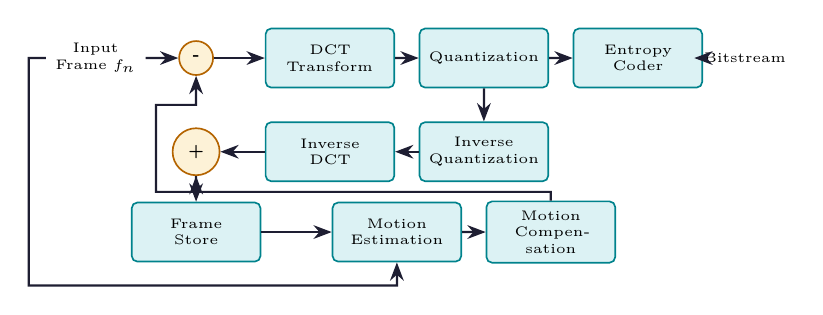
\begin{tikzpicture}[scale=0.85, every node/.style={font=\tiny}]
  \tikzset{
    sblock/.style={rectangle, draw=myteal, fill=hdrteal, text width=1.4cm,
      align=center, minimum height=0.75cm, font=\tiny,
      rounded corners=2pt, line width=0.6pt},
    junc/.style={circle, draw=myamber, fill=hdramber, minimum size=0.4cm,
      font=\tiny\bfseries, line width=0.6pt}
  }
  
  % Input frame
  \node (in) at (-1, 1.2) [align=center] {Input\\Frame $f_n$};
  
  % Sum junction to subtract prediction
  \node[junc] (diff) at (0.5, 1.2) {-};
  \draw[arrow] (in) -- (diff);
  
  % DCT
  \node[sblock] (dct) at (2.5, 1.2) {DCT\\Transform};
  \draw[arrow] (diff) -- (dct);
  
  % Quantization
  \node[sblock] (quant) at (4.8, 1.2) {Quantization};
  \draw[arrow] (dct) -- (quant);
  
  % Entropy Coder
  \node[sblock] (ent) at (7.1, 1.2) {Entropy\\Coder};
  \draw[arrow] (quant) -- (ent);
  
  % Output
  \node (out) at (8.7, 1.2) {Bitstream};
  \draw[arrow] (ent) -- (out);
  
  % Inverse Quantization
  \node[sblock] (iquant) at (4.8, -0.2) {Inverse\\Quantization};
  \draw[arrow] (quant) -- (iquant);
  
  % Inverse DCT
  \node[sblock] (idct) at (2.5, -0.2) {Inverse\\DCT};
  \draw[arrow] (iquant) -- (idct);
  
  % Reconstruction Summer
  \node[junc] (recon) at (0.5, -0.2) {+};
  \draw[arrow] (idct) -- (recon);
  
  % Frame Store
  \node[sblock] (store) at (0.5, -1.4) {Frame\\Store};
  \draw[arrow] (recon) -- (store);
  
  % Motion Estimation
  \node[sblock] (me) at (3.5, -1.4) {Motion\\Estimation};
  \draw[arrow] (store) -- (me);
  
  % Motion Compensation
  \node[sblock] (mc) at (5.8, -1.4) {Motion\\Compensation};
  \draw[arrow] (me) -- (mc);
  
  % Connections from Motion Compensation back to diff and recon
  \draw[arrow] (mc.north) |- (0.5, -0.8) -- (recon.south);
  \draw[arrow] (0.5, -0.8) -- (-0.1, -0.8) |- (0.5, 0.5) -- (diff.south);
  
  % Connection from Input frame to Motion Estimation
  \draw[arrow] (in.west) -- (-2.0, 1.2) |- (3.5, -2.2) -- (me.south);
\end{tikzpicture}
\end{tcolorbox}

\subsection{Video Standards}
\begin{itemize}[leftmargin=*, itemsep=3.5pt]
  \item \textbf{MPEG-1 / MPEG-2:} Formats used for VCDs ($MPEG-1$) and DVDs/Digital TV ($MPEG-2$).
  \item \textbf{H.264/AVC:} Incorporates intra-frame spatial prediction, quarter-pixel motion vector accuracy, and variable block sizes ($16\times16$ down to $4\times4$).
  \item \textbf{H.265/HEVC:} Replaces macroblocks with Coding Tree Units (CTUs) of size up to $64\times64$, reducing bitrates by $50\%$ compared to H.264 for equivalent quality.
\end{itemize}

% ===============================================================================
\section{Worked Examples}
% ===============================================================================

\begin{tcolorbox}[examplebox, title={Motion Vector Estimation}]
\textbf{Problem:} Given a $2 \times 2$ macroblock in the current frame $F_t$ and its corresponding search region in the reference frame $F_{t-1}$. Calculate the Mean Absolute Difference (MAD) for candidate displacement vectors $\mathbf{v}_1 = (0,0)$ and $\mathbf{v}_2 = (0,1)$, and identify the optimal motion vector.

\par\vspace{6pt}\noindent
\begin{minipage}{0.42\textwidth}
  \centering
  \textbf{Current Block $F_t$:}
  \[
    F_t = \begin{bmatrix} 80 & 85 \\ 70 & 75 \end{bmatrix}
  \]
\end{minipage}
\hfill
\begin{minipage}{0.53\textwidth}
  \centering
  \textbf{Reference Search Region $F_{t-1}$:}
  \par\vspace{4pt}
  \small
  \begin{tabular}{c | c c c}
    & $x=-1$ & $x=0$ & $x=1$ \\
    \hline
    $y=-1$ & 78 & 82 & 88 \\
    $y=0$  & 72 & \textbf{80} & \textbf{84} \\
    $y=1$  & 65 & \textbf{71} & \textbf{76}
  \end{tabular}
\end{minipage}
\par\vspace{6pt}

\par\noindent\rule{\linewidth}{0.5pt}\par
\textbf{Solution:}

\textbf{(a) For $\mathbf{v}_1 = (0,0)$:}
The candidate block in $F_{t-1}$ starting at $(0,0)$ is:
\[
  \begin{bmatrix} 80 & 84 \\ 71 & 76 \end{bmatrix}
\]
Compute the absolute differences:
\begin{align*}
  \text{Diff} &= \begin{bmatrix} |80 - 80| & |85 - 84| \\ |70 - 71| & |75 - 76| \end{bmatrix} = \begin{bmatrix} 0 & 1 \\ 1 & 1 \end{bmatrix} \\
  \text{MAD}(0,0) &= \frac{0 + 1 + 1 + 1}{4} = \frac{3}{4} = 0.75
\end{align*}

\textbf{(b) For $\mathbf{v}_2 = (0,1)$ (vertical shift by $j=1$):}
The candidate block in $F_{t-1}$ shifted by $(0,1)$ is:
\[
  \begin{bmatrix} F_{t-1}(0,1) & F_{t-1}(1,1) \\ F_{t-1}(0,2) & F_{t-1}(1,2) \end{bmatrix} = \begin{bmatrix} 71 & 76 \\ \text{N/A} & \text{N/A} \end{bmatrix}
\]
Since this candidate block contains out-of-bounds elements ($\text{N/A}$), we cannot calculate a valid MAD for $\mathbf{v}_2 = (0,1)$.

\par\vspace{6pt}
\textbf{Alternative Candidate Analysis:}
Let us analyze displacement $(i,j) = (-1,-1)$ (shifted top-left by 1 pixel) as an alternative candidate:
\begin{itemize}[leftmargin=*, itemsep=4pt]
  \item The candidate block in $F_{t-1}$ for $(i,j) = (-1,-1)$ is:
    \[
      \begin{bmatrix} F_{t-1}(-1,-1) & F_{t-1}(0,-1) \\ F_{t-1}(-1,0) & F_{t-1}(0,0) \end{bmatrix} = \begin{bmatrix} 78 & 82 \\ 72 & 80 \end{bmatrix}
    \]
  \item Compute the absolute differences with the current block $F_t$:
    \[
      \text{Diff} = \begin{bmatrix} |80 - 78| & |85 - 82| \\ |70 - 72| & |75 - 80| \end{bmatrix} = \begin{bmatrix} 2 & 3 \\ 2 & 5 \end{bmatrix}
    \]
  \item Calculate the MAD:
    \[
      \text{MAD}(-1,-1) = \frac{2 + 3 + 2 + 5}{4} = \frac{12}{4} = 3.00
    \]
\end{itemize}

\par\vspace{6pt}
\textbf{Conclusion and Motion Vector Selection:}
Comparing the calculated MAD values:
\begin{itemize}[leftmargin=*, itemsep=3pt]
  \item $\text{MAD}(0,0) = 0.75$
  \item $\text{MAD}(-1,-1) = 3.00$
\end{itemize}
Since $\text{MAD}(0,0) < \text{MAD}(-1,-1)$, the motion vector $\mathbf{v} = (0,0)$ is selected as the preferred motion vector.
\end{tcolorbox}

\newpage

% ===============================================================================
% MANDATORY QUICK REVISION PAGE
% ===============================================================================
\begin{center}
  {\large\bfseries\color{myred} Quick Revision --- Module VII}\\[3pt]
  {\small\color{mydark} Fundamentals of Video Coding $|$ PE-EC702B}
\end{center}
\noindent{\color{myred}\rule{\linewidth}{1.2pt}}
\vspace{4pt}

\begin{tcolorbox}[formulabox, title={\textbf{Key Formulas at a Glance}}]
\renewcommand{\arraystretch}{1.3}
\begin{tabularx}{\linewidth}{B{5.0cm} X}
Mean Absolute Difference & $\text{MAD}(i,j) = \frac{1}{N^2} \sum_{x=0}^{N-1} \sum_{y=0}^{N-1} \left| F_t(x,y) - F_{t-1}(x+i, y+j) \right|$ \\
Mean Squared Error & $\text{MSE}(i,j) = \frac{1}{N^2} \sum_{x=0}^{N-1} \sum_{y=0}^{N-1} \left[ F_t(x,y) - F_{t-1}(x+i, y+j) \right]^2$ \\
Search Complexity (Full) & $N_{\text{eval}} = (2p + 1)^2$ \quad ($p$ = search range) \\
Search Complexity (TSS) & $N_{\text{eval}} \approx 9 + 8 \log_2(p)$ \\
Motion Compensation Error & $e_t(x,y) = F_t(x,y) - F_{t-1}(x + dx, y + dy)$
\end{tabularx}
\tcbset{colbacktitle=myteal, coltitle=white}
\end{tcolorbox}

\begin{tcolorbox}[defbox, title={\textbf{One-Line Definitions}}]
\begin{itemize}[leftmargin=*, itemsep=2.5pt, topsep=0pt]
  \item \textbf{Motion Estimation:} The process of locating the displacement vector of a macroblock between successive video frames.
  \item \textbf{Motion Compensation:} The process of reconstructing a frame by shifting reference frame pixels using motion vectors.
  \item \textbf{I-Frame:} An intra-coded frame compressed independently using spatial details, acting as a random access sync point.
  \item \textbf{P-Frame:} A predicted frame coded using forward temporal prediction from a single preceding reference frame.
  \item \textbf{B-Frame:} A bidirectional frame coded using both past and future reference frames, offering maximum compression.
  \item \textbf{GOP:} Group of Pictures, defining the recurring sequence pattern of I, P, and B frames in a video stream.
\end{itemize}
\end{tcolorbox}

\begin{tcolorbox}[exambox, title={\textbf{Frequently Asked / Viva Questions}}]
\begin{enumerate}[leftmargin=*, itemsep=3.5pt, label=\arabic*.]
  \item \Q{What is temporal redundancy in video coding?} It is the high correlation between consecutive frames in a video sequence, where background and moving objects remain mostly identical from frame to frame.
  \item \Q{How does the Hybrid Video Encoder combine spatial and temporal compression?} It uses motion estimation (temporal prediction) to generate a residual prediction error, which is then compressed using 2D DCT and quantization (spatial transform coding).
  \item \Q{Why do B-frames achieve much higher compression than P-frames?} Because B-frames use bidirectional prediction, meaning they can reference macroblocks from both past and future frames, yielding smaller prediction errors.
  \item \Q{What is the trade-off of using a large number of B-frames in video streaming?} B-frames require future frames to be decoded first, which introduces frame buffering delay (latency) and increases decoder memory requirements.
  \item \Q{Explain the Three-Step Search (TSS) algorithm.} It is a fast search method that evaluates 9 points using a coarse step size, shifts the center to the minimum error point, halves the step size, and repeats until the step size is 1.
  \item \Q{What is a macroblock in video standards?} A macroblock is a $16 \times 16$ pixel region of luminance (Y) along with the corresponding chrominance (U, V) blocks, representing the basic processing unit for motion compensation.
  \item \Q{State the main advantage of H.264/AVC over MPEG-2.} H.264/AVC achieves comparable visual quality at approximately half the bitrate of MPEG-2 by using intra-prediction, multi-frame references, and variable block sizes.
  \item \Q{What are CTUs in H.265/HEVC?} Coding Tree Units (CTUs) replace macroblocks in H.265. They can be dynamically partitioned into Coding Units (CUs) from $64 \times 64$ down to $8 \times 8$, optimizing compression for high-resolution (4K/8K) video.
  \item \Q{Why are P-frames and B-frames unsuitable as random access entry points?} Because they contain temporal prediction residuals, meaning they cannot be decoded without first decoding their past and future reference frames.
  \item \Q{Define the Motion Vector.} The displacement vector $(dx, dy)$ representing the horizontal and vertical offset of a matching block in the reference frame relative to the current frame.
\end{enumerate}
\tcbset{colbacktitle=myteal, coltitle=white}
\end{tcolorbox}

\begin{tcolorbox}[tikzbox, title={Comparison of Video Frame Types}]
\centering
\renewcommand{\arraystretch}{1.2}
\begin{tabularx}{\linewidth}{>{\bfseries}B{3.2cm} Y Y Y}
\rowcolor{hdrgray} Attribute & I-Frame (Intra) & P-Frame (Predicted) & B-Frame (Bidirectional) \\
\midrule
Coding Source & Self-contained (spatial) & Temporal (forward) & Temporal (bidirectional) \\
\rowcolor{rowalt} Compression Ratio & Low ($2:1$ to $5:1$) & Moderate ($10:1$ to $20:1$) & High ($30:1$ to $50:1$) \\
Random Access Point & Yes & No & No \\
\bottomrule
\end{tabularx}
\tcbset{colbacktitle=myteal, coltitle=white}
\end{tcolorbox}

\end{document}
